\documentclass{article}
\usepackage[utf8]{inputenc}
\usepackage{geometry}
\usepackage{indentfirst}
\usepackage{hyperref}
 \geometry{
 a4paper,
 total={170mm,257mm},
 left=20mm,
 top=20mm,
 }
 \usepackage{graphicx}
 \usepackage{titling}
\renewcommand{\figurename}{Şekil}
 \title{Yapay Zekâ Destekli Robotlar ile Arama Kurtarma Çalışmaları}
\author{Turhan Can KARGIN}
\date{Mart 2023}
 
 \usepackage{fancyhdr}
\fancypagestyle{plain}{%  the preset of fancyhdr 
    \fancyhf{} % clear all header and footer fields
    \fancyfoot[R]{
\includegraphics[width=3cm]{Images/globalai.png}}
    \fancyfoot[L]{\thedate}
    \fancyhead[L]{\textbf{Konu:} Deprem Sonrasında Oluşan Sorunları Azaltmak için bir Proje Fikri}
    \fancyhead[R]{\theauthor}
}
\makeatletter
\def\@maketitle{%
  \newpage
  \null
  \vskip 1em%
  \begin{center}%
  \let \footnote \thanks
    {\LARGE \@title \par}%
    \vskip 1em%
    %{\large \@date}%
  \end{center}%
  \par
  \vskip 1em}
\makeatother

\usepackage{lipsum}  
\usepackage{cmbright}

\begin{document}

\maketitle

\noindent\begin{tabular}{@{}ll}
    \textbf{Proje Sahibi} & \theauthor\\
    \textbf{Proje Destekleyicisi} & Global AI Hub
\end{tabular}

\section*{Özet}
Deprem sonrası en kritik konulardan biri, enkaz altında kalan insanların kurtarılmasıdır. Yapay zekâ destekli robotlar, insanların ulaşamayacağı bölgelere ulaşarak kurtarma çalışmalarına destek sağlayabilirler. Bu sunum, deprem sonrası kurtarma çalışmalarına yardımcı olmak için yapay zekâ destekli robotların kullanımını hakkında sunulabilecek fikirleri ele almaktadır. Yapay zekâ destekli robotlar, afet bölgesinde birçok görevi yerine getirebilirler ve insanların güvenliğini riske atmadan tehlikeli ve zorlu ortamlarda çalışabilirler. Ayrıca, sağlık çalışanlarının da yardımcısı olabilirler. Bu sunumda, yapay zekâ destekli robotların kullanımının avantajları ve eksiklikleri tartışılmaktadır.

\begin{figure}[h]
\centering
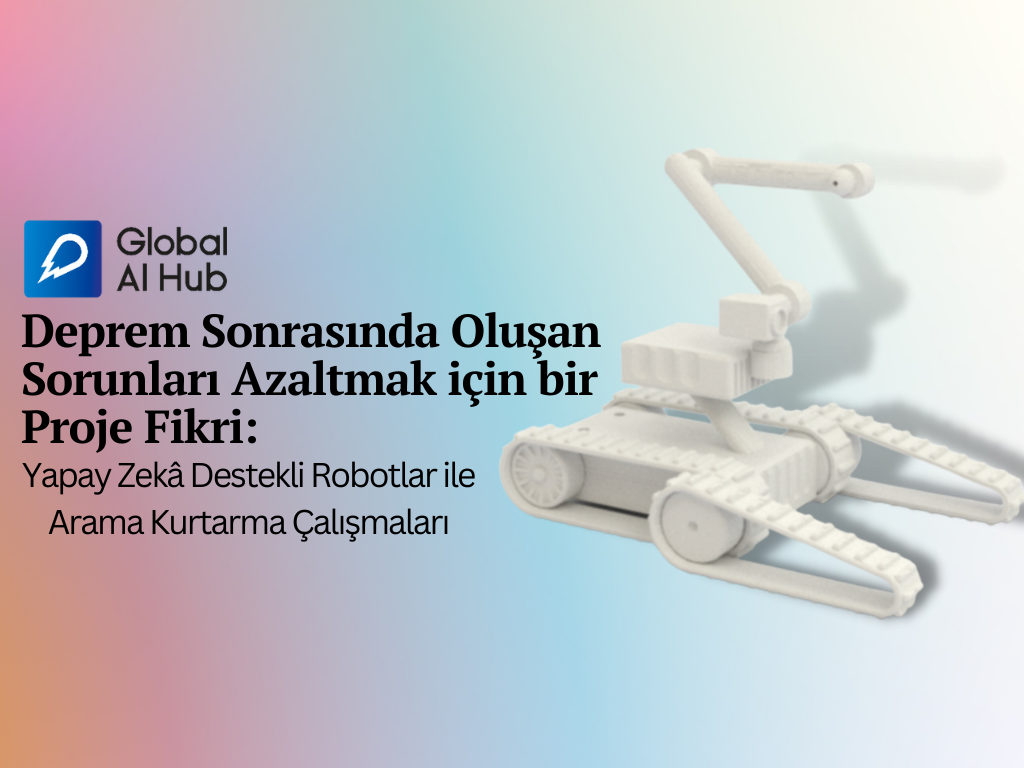
\includegraphics[width=1\textwidth]{Images/baslik.png}
\caption{Başlık Görseli}
\end{figure}

\section*{Yapay zekâ destekli robot teknolojilerinin afet kurtarma çalışmalarında kullanımı}
Bildiğiniz gibi 6 şubat 2023 tarihinde Kahramanmaraş’ta meydana gelen iki büyük deprem sonrasında yapılan arama kurtarma çalışmaları çok efektif bir şekilde ilerlememiştir. Organize arama kurtarma çalışmalarında bir çok problem meydana gelmiştir. İleride bunar benzer sorunlar yaşamamak için yapay zekâ destekli robot teknolojileri, afet kurtarma çalışmalarında insanların güvenliğini ve hayatlarını korumak için çok faydalı olabilir. Bu robotlar, insanların güvenliğini riske atmadan tehlikeli ve zorlu ortamlarda çalışabilirler. Ayrıca, insanlar tarafından erişilemeyen yerlere de kolaylıkla ulaşabilirler. Yapay zekâ destekli robotlar, bir afet bölgesinde birçok görevi yerine getirebilirler. Örneğin, hasarlı yapıların içindeki insanları tespit etmek, su baskınlarında suların yönünü ve seviyesini belirlemek, enkaz yığınlarının altında kalan insanları tespit etmek ve kurtarmak gibi birçok görevde kullanılabilirler. Ayrıca, sağlık çalışanlarının da yardımcısı olabilirler. Örneğin, yaralıları taşımak, ilk yardım malzemeleri ve ilaçları taşımak, tıbbi cihazları taşımak gibi görevlerde de kullanılabilirler. Yapay zekâ destekli robot teknolojilerinin kullanımı, afet kurtarma çalışmalarının hızını arttırabilir. Robotlar, insanların yapması gereken zorlu görevleri yerine getirerek insanların zamanını ve enerjisini tasarruf ederler. Ayrıca, robotlar 24 saat çalışabilirler ve insanlar tarafından erişilmesi zor olan yerlerde bile çalışabilirler. Tüm bunların yanı sıra, yapay zekâ destekli robotlar, afet kurtarma çalışmalarında insanların güvenliğini sağlayarak, insan hayatlarını kurtarma konusunda çok önemli bir rol oynayabilirler. Robotlar afet müdahale ve kurtarma çalışmalarında önemli bir rol oynayabilir. Teknoloji bu yönde gelişiyor, ancak bu teknolojiyi kullanma isteği henüz Türkiye’de hatta hiçbir ülkede daha oluşmadı. Bu sunumun ilerleyen kısımlarında bu teknolojinin eksiklerini ve bu eksikliklerin nasıl giderilebileceğine dair detaylar paylaşacağım.
\\ \\
Robotlar afetler sırasında molozları eleyerek veya bir depremden sonra mahsur kalanlara hayat kurtaran malzemeler ulaştırarak değerli araçlar olarak görev yapabilir. İnsansız sistemler değerli keşifler sağlayabilir ve her geçen dakikanın hayatta kalma açısından sonuçlar doğurduğu senaryolar olan sel veya yangınlar sırasında müdahale sürelerini hızlandırmak için tehlikeli veya bilinmeyen ortamlara sızabilir. Afet müdahale ve kurtarma çalışmalarına yardımcı olmak üzere robotların benimsenmesi son derece yavaş gerçekleşmektedir bu sunumda bunların nedenleri ve potansiyel çözün yolları tartışılacaktır. 

\begin{figure}[h]
\centering
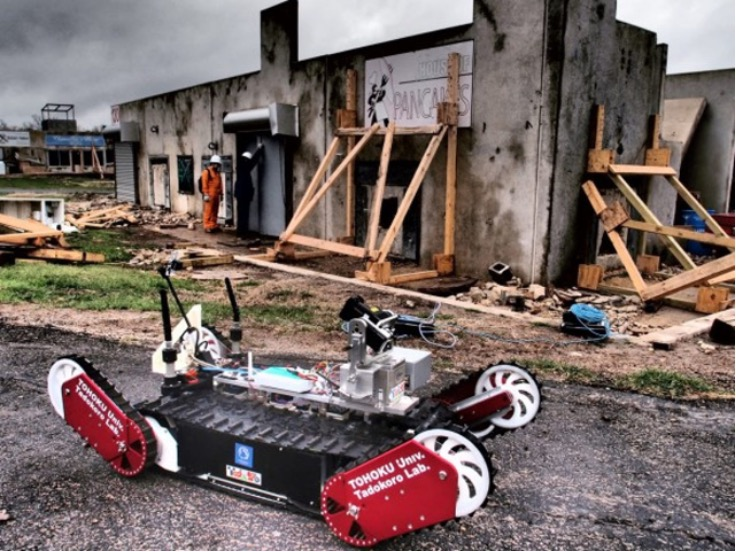
\includegraphics[width=0.75\textwidth]{Images/Resim1.jpg}
\caption{Tohoku Üniversitesi tarafından test edilen bir afet sonrası kurtarma robotu}
\end{figure}

\section*{Literatür ve Projeler}
\begin{itemize}
    \item Scanlan J, Flynn D, Lane DM, Richardson R, Richardson T, Sóbester A. Extreme Environments Robotics: Robotics for Emergency Response, Disaster Relief and Resilience. UK-RAS Network, 2017. 28 p. (UK-RAS White Papers).
    \item Chitikena H, Sanfilippo F, Ma S. Robotics in Search and Rescue (SAR) Operations: An Ethical and Design Perspective Framework for Response Phase. Applied Sciences. 2023; 13(3):1800.
    \item Disaster Robotics By Robin R. Murphy (MIT Press)
    \item Quince: Şiddetli bir afet nedeniyle kısmen çökmüş bir binayı veya yeraltı tesisini araştıran bir Robotik Sistem (Tohoku Universitesi)
    \item MIT tarafından geliştirilen iRobot robotu
    \item ABD'de kullanılan insansız hava araçları (İHA) ile yangın söndürme, Japonya'da kullanılan insansı robotlar ile bina enkazı altında kalan insanların kurtarılması
    \item Japonya, Fukuşima'da moloz temizlemek için sekiz uzuvlu bir 'ahtapot' robot geliştirilmesi.
\end{itemize}

\begin{figure}[h]
\centering
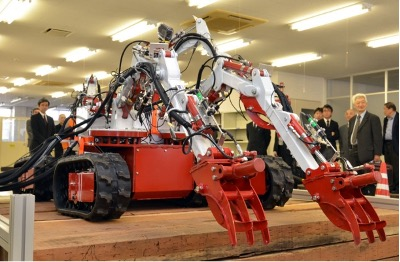
\includegraphics[width=0.75\textwidth]{Images/Resim2.jpg}
\caption{Ahtapot robotu (Waseda University)}
\end{figure}

\section*{Eksikler}
Yapay Zekâ Destekli Kurtarma Çalışmaları konusunda yapılan projeler, teknolojik gelişmelere rağmen hala birçok eksiklik barındırmaktadır. Bu eksiklikler şunlar olabilir:
\begin{itemize}
    \item Donanım Eksiklikleri: Yapay zekâ destekli robotların kullanımı, yüksek teknolojili donanımların gerektirmektedir. Fakat, bu donanımların çoğu pahalıdır ve her yerde bulunmayabilir. Bu nedenle, afet bölgelerine hızlı ve etkili bir şekilde müdahale edilmesi zorlaşabilir.
    \item Veri Kalitesi Sorunları: Yapay zekâ teknolojileri, doğru ve güvenilir verilere ihtiyaç duyar. Ancak, afet bölgelerinde veri toplamak ve analiz etmek zor olabilir. Bu nedenle, yanlış veya eksik verilerin kullanılması, kurtarma çalışmalarının etkinliğini azaltabilir.
    \item Güvenlik Sorunları: Yapay zekâ destekli kurtarma çalışmaları sırasında, insanlarla robotların işbirliği içinde çalışması gerekebilir. Bu durumda, güvenlik sorunları ortaya çıkabilir ve robotların insanlara zarar verme riski olabilir.
    \item Etik Sorunlar: Yapay zekâ destekli kurtarma çalışmaları, bazı etik sorunları da beraberinde getirebilir. Örneğin, insansız hava araçları ile gerçekleştirilen kurtarma çalışmaları, özel hayatın gizliliği konusunda sorunlar yaratabilir.
\end{itemize}
Bu eksiklikler, yapay zekâ destekli kurtarma çalışmalarının uygulanmasını zorlaştırabilir. Bu nedenle, bu teknolojilerin geliştirilmesi ve uygulanması sırasında bu eksikliklerin göz önünde bulundurulması gerekmektedir.

\section*{Çözüm}
Yapay Zekâ Destekli Kurtarma Çalışmaları konusundaki eksikliklerin giderilmesi için birkaç çözüm önerisi şunlar olabilir:
\begin{itemize}
    \item Donanım Eksiklikleri: Donanım maliyetlerinin düşürülmesi için, yapay zeka destekli robotların modüler bir tasarıma sahip olması ve birçok farklı görev için kullanılabilmesi gereklidir. Ayrıca, yerel üretim veya üretimde kullanılmış malzemelerin geri dönüştürülmesi gibi alternatifler de düşünülebilir.
    \item Veri Kalitesi Sorunları: Veri kalitesi sorunlarının giderilmesi için, afet öncesi ve sonrası dönemde veri toplama ve yönetim sistemlerinin kurulması gereklidir. Bu veriler hem insanlar hem de yapay zeka algoritmaları tarafından analiz edilebilir. Ayrıca, veri analizinde güvenilir ve doğru sonuçlar elde etmek için veri doğruluğunu artırmaya yönelik teknolojiler geliştirilebilir.
    \item Güvenlik Sorunları: Robotların insanlarla güvenli bir şekilde çalışabilmesi için, insanların robotlar hakkında yeterli bilgiye sahip olması gereklidir. Bu nedenle, robotlar ve insanlar arasındaki etkileşimi sağlamak için eğitim ve bilgilendirme kampanyaları düzenlenebilir. Ayrıca, robotlar için güvenlik önlemleri geliştirilebilir ve robotların insanları algılaması ve onlardan kaçınması için sensörler kullanılabilir.
    \item Etik Sorunlar: Yapay zeka destekli kurtarma çalışmaları sırasında ortaya çıkan etik sorunları ele almak için, hukuki düzenlemeler yapılabilir. Özellikle, veri gizliliği ve özel hayatın korunması konularında hukuki düzenlemeler yapılması gereklidir. Ayrıca, robotların insanlarla etkileşimleri sırasında etik kurallara uyulması için robotlar için etik kuralları belirleyen standartlar oluşturulabilir. Örneğin, Avrupa Birliği'nin Genel Veri Koruma Yönetmeliği (GDPR), İngiltere'nin robotik ve yapay zeka etik kodu.
\end{itemize}
Bu çözüm önerileri, yapay zeka destekli kurtarma çalışmalarının eksikliklerinin giderilmesine yardımcı olabilir ve bu teknolojilerin daha etkili bir şekilde kullanılmasına olanak sağlayabilir.

\begin{figure}[h]
\centering
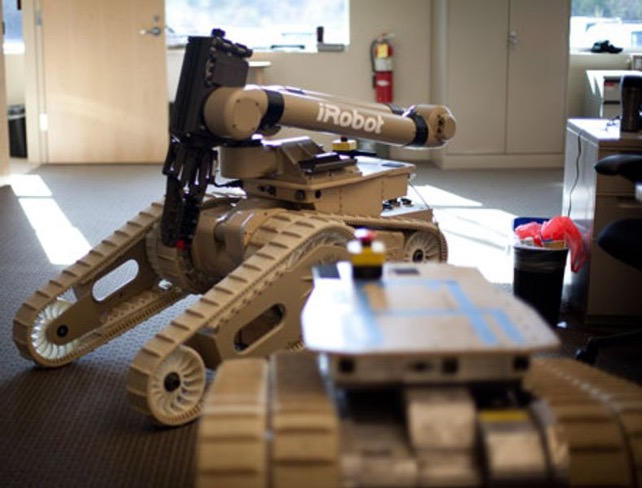
\includegraphics[width=0.75\textwidth]{Images/Resim3.jpg}
\caption{iRobot}
\end{figure}

\section*{Sonuç}
Yapay zekâ destekli robotlar, deprem sonrası kurtarma çalışmalarında insanların hayatını kurtarmak için çok faydalı olabilirler. Bu teknolojilerin gelecekte afet kurtarma çalışmalarında daha yaygın bir şekilde kullanılması ile, insan hayatlarını kurtarma ve yıkımı en aza indirgeme konusunda daha etkili sonuçlar elde edilebilir. Robotlar, afet bölgesinde birçok görevi yerine getirerek insanların zamanını ve enerjisini tasarruf ederler. Ayrıca, robotlar insanların güvenliğini sağlayarak, afet müdahale ve kurtarma çalışmalarında önemli bir rol oynayabilirler. Ancak, bu teknolojinin eksiklikleri de vardır. Örneğin, robotların hareket kabiliyeti sınırlı olabilir ve bazı görevleri yerine getiremeyebilirler. Ayrıca, robotların maliyeti de yüksek olabilir. Bu sunumda, yapay zekâ destekli robotların avantajları ve eksiklikleri tartışılmıştır. Bu eksikliklerin giderilmesi için daha fazla araştırma yapılması gerektiği ve robotların afet kurtarma çalışmalarında kullanımının yaygınlaştırılması için çaba sarf edilmesi gerektiği sonucuna varılmıştır.

\section*{Kaynaklar}
\begin{itemize}
    \item \href{https://www.youtube.com/watch?v=wG4RnDNWtJo}{These Robots Come to the Rescue after a Disaster | Robin Murphy | TED Talks}.
    \item \href{https://www.zdnet.com/article/disaster-robots-slow-to-gain-acceptance-from-responders/}{Disaster robots slow to gain acceptance from responders}
    \item \href{https://spectrum.ieee.org/irobot-sending-packbots-and-warriors-to-fukushima}{iRobot Sending Packbots and Warriors to Fukushima Dai-1 Nuclear Plant}
    \item \href{https://www.kisiselverilerinkorunmasi.org/mevzuat/avrupa-birligi-genel-veri-koruma-tuzugu-gdpr-turkce-ceviri/}{Avrupa Birliği Genel Veri Koruma Tüzüğü (GDPR)}
    \item \href{https://www.gov.uk/guidance/understanding-artificial-intelligence-ethics-and-safety}{Understanding artificial intelligence ethics and safety}
\end{itemize}

\end{document}
